\section{Motivation}
\label{s:motivation}

This work is motivated by an observation that prior approaches
focus on the execution order of a single pair of conflicting
accesses, but race conditions mostly are \textit{combined results of multiple pairs} 
of conflicting accesses.
%
Because of this gap\yj{xx}, prior approaches shows inefficiency in finding race
conditions.

In this section, we first describe when and how race conditions
manifest to comprehend what interleavings should be tested to find
race conditions.
%
Afterwards, we identify why prior approaches are limited in finding
race conditions, and clarify our goals to address the limitations.


\PP{Manifestation of race conditions}
%
According to an extensive survey of concurrency
bugs~\cite{learningfrommistakes}, most race conditions manifest
depending on the execution order of multiple memory access operations.
%
Specifically, the study identifies that 92\% of race conditions manifest 
when at most four memory accesses operations are executed in a specific
order.

\dr{need to more emphasize this throughout the motivation section:}
Furthermore, a few literatures~\cite{pctalgorithm, ski, snorlax,
  failuresketching} imply that the number of \textit{scheduling
  constraints} for most race conditions is small.
%
A scheduling constraint indicates an ordering constraint between a
single pair of instructions executed different threads, such that an
instruction \texttt{X} is executed before \texttt{Y} (denoted as
$\texttt{X} \rightarrow \texttt{Y}$).
%
In terms of scheduling constraint, a race condition manifests if a
\textit{conjunction of a small number of scheduling constraints} are
simultaneously satisfied.
%
\dr{}
%
Specifically, race conditions that the above literatures study
manifest with at most two scheduling constraints.



\begin{figure}[t]
  \centering
  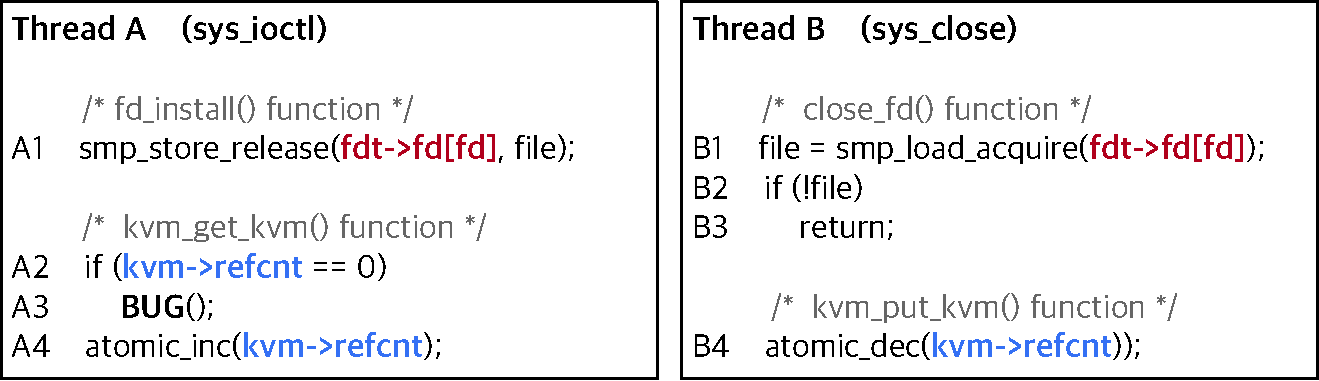
\includegraphics[width=0.95\linewidth]{fig/cve-2017-10661.pdf}
  \caption{Simplified code snippet of a NULL-dereference bug in the
    binder driver.}
  \label{fig:cve-2019-6974}
\end{figure}

To illustrate the manifestation of race conditions,
\autoref{fig:cve-2019-6974} describes a race condition occured in the
binder device driver, which is an IPC framework for
Android. Specifically, a NULL-dereference bug manifests when two
system calls are executed concurrently: \texttt{mmap()} to map the
device driver into a user address space and
\texttt{ioctl(TRANSACTION)} to send an IPC message.
 

% \yj{Are you talking about \autoref{fig:alias-coverage}?}
The race condition manifests depending on four memory accesses,
\texttt{A1} and \texttt{A2} in thread~A, and \texttt{B1} and
\texttt{B4} in thread~B. Let us suppose \texttt{alloc->vma} and
\texttt{alloc->mm} are initially \texttt{NULL}.
%
During mapping the device driver into a user address space, thread~A
sets \texttt{alloc->vma} and \texttt{alloc->mm} to non-NULL pointers
at \texttt{A1} and \texttt{A2}.
%
However, since these two store operations are not atomically executed,
thread~B may intervene in the middle of these two operations.
%
In that case, if \texttt{A1} is executed before \texttt{B1}, thread~B
does not return at \texttt{B3} because thread~B reads a non-NULL
pointer value through \texttt{alloc->vma}.
%
And then if \texttt{B4} is executed before \texttt{A2},
\texttt{alloc->mm} still remains \texttt{NULL} when thread~B
increments the reference counter of \texttt{alloc->mm} at \texttt{B4},
causing a NULL-dereference bug.

In this example, we can confirm that the manifestation of the race
condition follows the implications of previous studies; the race
condition manifests if \textit{two} scheduling constraints on
\textit{four} memory access operations (\ie,
$(\texttt{A1} \rightarrow \texttt{B1}) \wedge (\texttt{B4} \rightarrow
\texttt{A2})$) are conjunctively satisfied.


% One of the factors that makes it difficult to find concurrency bugs is
% that, they may be detected only when a program shows an abnormal
% behavior.
% %
% \autoref{subfig:racecondition} is the example of such concurrency bug.
% %
% In this example, the timing of accesses are not correctly
% contemplated. When instructions are executed in the order of
% \dr{TODO:}..., the program runs differently than the developer
% intention, causing a use-after-free bug.
% %
% However there are no plain accesses (\ie, all accesses are annotated),
% and therefore, there is no data race.
% %
% By the definition, data race detectors~\cite{tsan, kcsan, krace,
%   prorace, txrace, crsampler} are not applicable to detect this kind
% of race conditions.


% In worse cases, race conditions hardly manifest with the kernel
% scheduler. In detail, a race condition may manifest only when one
% thread stalls for a long time while another thread executes numerous
% instructions.
% %
% One could argue that those concurrency bugs are not a threat because
% it may take too long time, or even impossible to exploit.
% %
% However, a recent study, ExpRace~\cite{exprace}, reveals that an
% attacker can affect the kernel's scheduler using inter-processor
% interrupts (IPI), and exploit even such concurrency bugs.



\PP{Limitation of existing approaches}
%
In the perspective of fuzzing, a coverage metric is a paramount gear
to determine whether a given input is worthy of further mutation.
%
If a coverage metric does not represent whether an input has a
potential to trigger a race condition, a fuzzer may ignore inputs in
which there are unexplored interleavings, or waste the computing power
to valueless inputs.
%
In this regard, our primary question is whether existing coverage
metrics in the concurrency dimension are suitable to apprehend
interleavings potentially causing a race condition, for example,
$(\texttt{A1} \rightarrow \texttt{B1}) \wedge (\texttt{B4} \rightarrow
\texttt{A2})$ in \autoref{fig:cve-2019-6974}.



Unfortunately, we observe that none of existing approaches incorporate
a proper coverage metric for race conditions.
%
A few of existing approaches~\cite{snowboard, razzer} do not adopt a
coverage in the concurrency dimension at all. Therefore, they do not
make a decision as to whether a given input is worth further testing.
%
Other approaches~\cite{krace, muzz} adopt coverage metrics that are
not suitable for race conditions as they do not consider a combined
result of multiple pairs of conflicting accesses. As a consequence,
race conditions may not be exposed even after the coverages are
saturated.
%
% Consequently, existing approaches have difficulty in distinguishing a
% given input has a potential to cause an interesting behavior, \ie,
% a race condition.


\begin{figure}[t]
  \centering
  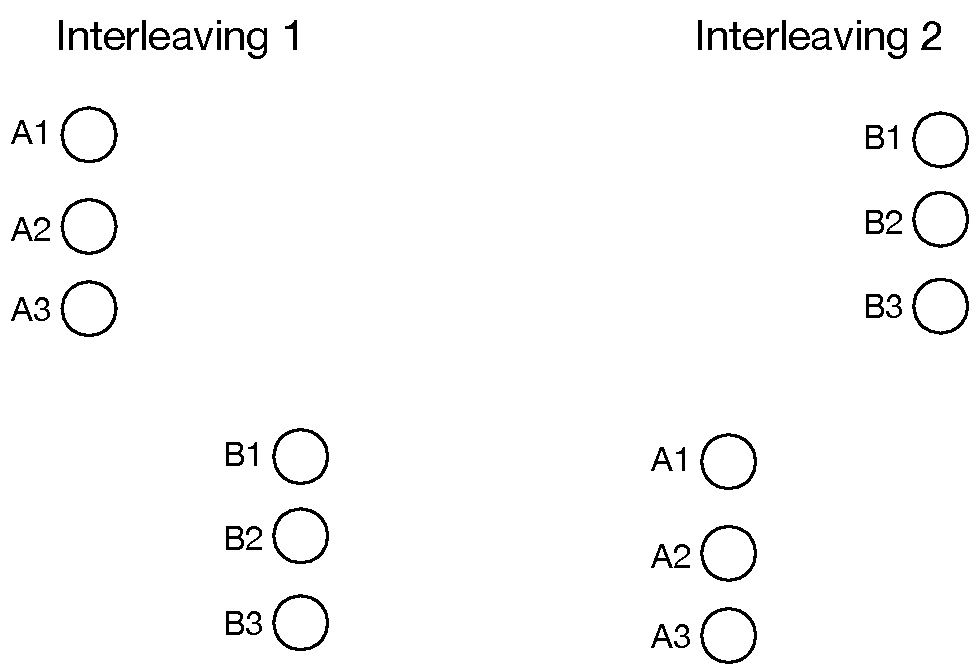
\includegraphics[width=0.98\linewidth]{fig/alias-coverage.pdf}
  \caption{Three inputs that consist of two concurrent syscalls. For
    all inputs, thread~A executes the same \texttt{mmap()} syscall
    while thread~B handles different ioctl requests. For brevity, we
    describe only conflicting instructions.\dr{Change the name of two
      ioctls in input 1 and 2}}
  \label{fig:alias-coverage}
\end{figure}

\yj{This is the key paragraph to point out the limitation of previous approaches, but very vague. Make specific claims of why Kraces' alias coverage is insufficient by giving an example.}
%
In order to show why comprehending multiple pairs of conflicting
accesses is important, let us suppose we have three inputs that
consists of two concurrent syscalls as described in
\autoref{fig:alias-coverage}.
%
For all inputs, thread~A executes a \texttt{mmap()} syscall to map the
binder driver to a user address space while thread~B handles different
ioctl requests such that \texttt{ioctl(FREE_BUFFER)},
\texttt{ioctl(REPLY)}, and \texttt{ioctl(TRANSACTION)} for
\texttt{Input 1}, \texttt{Input 2}, and \texttt{Input 3} respectively.
%
It is worth noting that in \texttt{Input 1} and \texttt{Input 2},
there is only one pair of conflicting accesses; in \texttt{Input 1},
the two threads conflict on \texttt{alloc->vma}, and in \texttt{Input
  2}, the two threads conflict on \texttt{alloc->mm}.



\begin{figure}[t]
  \centering
  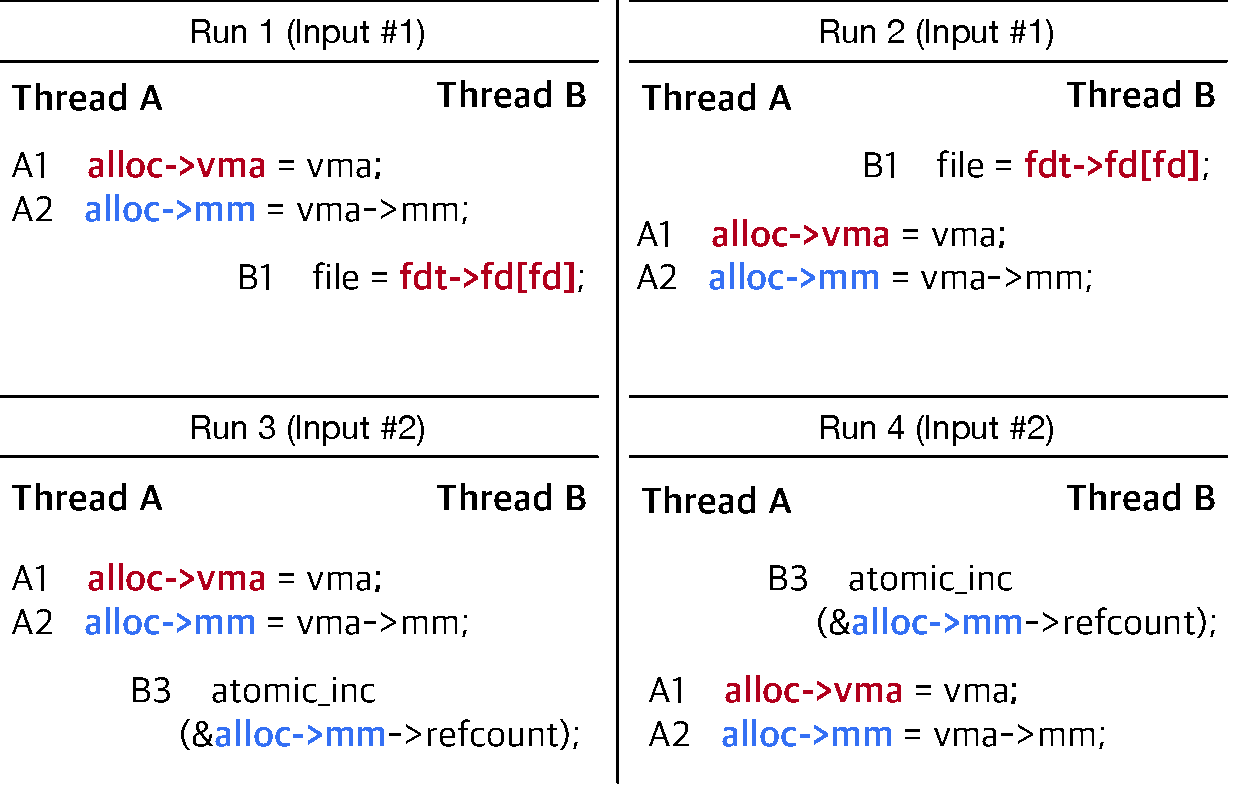
\includegraphics[width=0.9\linewidth]{fig/alias-coverage-interleaving.pdf}
  \caption{Four interleavings of \texttt{Input 1} and \texttt{Input 2}
    in \autoref{fig:alias-coverage}. After executing these four
    interleavings, all possible execution orders of a single
    conflicting accesses are exhibited.\dr{Run 1 -> Interleaving 1?}}
  \label{fig:alias-coverage-interleaving}
\end{figure}

In this example, if we adopt a coverage metric that focuses on a
single pair of conflicting accesses (\eg, alias coverage), a fuzzer
may not recognize that \texttt{Input 3} may exhibit a behavior
different than \texttt{Input 1} and \texttt{Input 2}~(\ie, a
NULL-dereference bug).
%
\autoref{fig:alias-coverage-interleaving} shows four interleavings
that exhibits all execution order of a single pair of conflicting
accesses. If a fuzzer executes \texttt{Input 1} with interleavings in
\texttt{Run 1} and \texttt{Run 2}, a fuzzer observes execution orders
such as $\texttt{A1} \rightarrow \texttt{B1}$ (in \texttt{Run 1}) and
$\texttt{B1} \rightarrow \texttt{A1}$ (in \texttt{Run 2}).
%
Similary, if a fuzzer executes \texttt{Input 2} with interleavings in
\texttt{Run 3} and \texttt{Run 4}, it observes execution orders of
$\texttt{A2} \rightarrow \texttt{B4}$ (in \texttt{Run 3}) and
$\texttt{B4} \rightarrow \texttt{A2}$ (in \texttt{Run 4}).
%
After executing these four interleavings, \texttt{Input 3} does not
reveal a new execution order of a single conflicting
accesses. Therfore, as a Krace state, a fuzzer may de-prioritize
\texttt{Input 3}, and the race condition may not be found.

In summary, in order to determine whether an input shows interesting
behaviors or not, a fuzzer needs to comprehend \textit{a combined
  result of multiple pairs of conflicting accesses} as it is the
primary reason of race conditions.


\cut{
Approaches that adopt a randomized scheduler~\cite{krace, ski, muzz}
suffer from the inherent randomness.
%
When the randomness comes to concurrency bugs, this could become a
significant drawback.
%
Although interleavings are affected by a fuzzer, a fuzzer cannot fully
control how interleaving takes place. Thus, a fuzzer may need to
indiscriminately execute the same input until its coverage is
saturated.
%
Furthermore, it is almost impossible for randomized schedulers to
expose concurrency bugs requiring an extreme interleaving such that
\dr{TODO: explain:}non-inclusive race conditions~\cite{exprace} or ones that
require a very small race window.
%
In contrast, approaches with a hint-directed scheduler is able to
explore all interelavings including even ones that hardly occur if a
proper scheduling hint is given. Therfore, they are able to find out
such race conditions.
%
However, existing approaches~\cite{razzer, snowboard} are not suitable
of diversifying interleavings. \ie, they change very small part of
interleaving across runs.
%
Even with a single input, they require a large number of execution to
test the input enough.
}

\PP{Our goal}
%
Our goal is to design a fuzzer to explore the interleaving space with
a purpose of effectively testing conjunctions of scheduling
constraints.
%
% Considering characteristics of concurrency bugs mentioned above, it
% will increase the probabilty of finding more concurrency bugs if we
% diversify interleavings to experience such partial orders as many as
% possible.

To this end, we organize subgoals as follows:
%
1) We first design a coverage metric to track conjunctions of
scheduling constraints,
%
2) based on the coverage metric, we design an instruction scheduling
algorithm that quickly saturate the coverage metric, and lastly,
%
3) we combine the coverage metric and the instruction scheduling
algorithm into Syzkaller~\cite{syzkaller} to find out race conditions
in the Linux kernel.



%%% Local Variables:
%%% mode: latex
%%% TeX-master: "p"
%%% End:
